\documentclass[aps,pra,twocolumn,reprint,amsmath,amssymb]{revtex4-2}

\usepackage{graphicx}
\usepackage{booktabs}
\usepackage{siunitx}
\usepackage[colorlinks=true,linkcolor=blue,citecolor=blue,urlcolor=blue]{hyperref}

\usepackage{xcolor}
\graphicspath{{../figures/}}

\begin{document}

\title{Gray-Box Adaptive Control for Circuit QED Systems}
\author{JianJun}
\affiliation{Shyam Shankar Quantum Circuits Group}
\date{\today}

\begin{abstract}
Model mismatch is a practical bottleneck for pulse-level control in circuit quantum
electrodynamics (cQED), especially when gradient-based pulse optimization is sensitive to an
incorrect dispersive shift $\chi$. This study evaluates a gray-box workflow in which a
multi-Fock Ramsey probe estimates the true $\chi$, after which gradient ascent pulse
engineering (GRAPE) is rerun on the corrected learner model. Using the consolidated
\texttt{cqed\_sim}-based study pipeline, we compare nominal, gray-box, perfect-knowledge, and
black-box control strategies for a simultaneous qubit $X$ gate across Fock sectors
$n=0,1,2,3$. The main benchmark is a 30\% $\chi$ mismatch between learner and truth models,
with additional sweeps over mismatch level, decoherence, readout confusion, finite shot
budget, slow drift, and omitted higher-order Hamiltonian terms. Gray-box correction raises
the noiseless truth-model fidelity from $0.8990$ to $0.9541$ at 30\% mismatch, recovering
99.8\% of the perfect-model performance gap, while a model-free black-box baseline reaches
only $0.8877$ after 1394 truth-model evaluations. The improvement remains stable over a
70\% mismatch sweep, survives readout confusion up to 15\%, and continues to outperform the
nominal strategy under decoherence and slow drift. Fresh validation checks confirm that the
main conclusion is stable under modest Hilbert-space enlargement and expanded multistart
optimization. The repository now contains a reproducible validator, compiled report, and an
updated improvement log for future gray-box extensions.
\end{abstract}

\maketitle

\section{Introduction}

Dispersive qubit-cavity control is central to bosonic quantum information processing in cQED,
where high-fidelity gates depend on an accurate Hamiltonian model of the transmon-cavity
system \cite{koch2007,blais2021}. This sensitivity is particularly acute for GRAPE-style
optimal control \cite{khaneja2005}, because the optimizer exploits coherent phase
accumulation over many time slices. If the learner model uses an incorrect dispersive shift
$\chi$, a pulse that is nearly optimal on the training Hamiltonian can underperform badly on
the physical device.

Adaptive control offers a middle ground between fully model-based and fully model-free
optimization. In the hybrid approach of Egger and Wilhelm \cite{egger2014}, targeted
measurements update a structured model before the next optimization round. Randomized
benchmarking-based adaptation similarly uses measurement feedback to steer control parameters
toward better performance \cite{kelly2014}. The present study asks whether a similar gray-box
strategy is viable in a dispersive cQED setting, where the uncertain quantity is the
qubit-cavity dispersive shift and where the probe itself can be designed around known
Hamiltonian structure.

The concrete task is a simultaneous qubit $X$ gate on the logical block
$\{|g,n\rangle, |e,n\rangle\}_{n=0}^{3}$. We compare four strategies: nominal GRAPE on the
mis-specified learner model, gray-box GRAPE after a multi-Fock Ramsey probe, perfect-knowledge
GRAPE, and a model-free black-box baseline. The study also probes robustness to finite shots,
readout confusion, decoherence, slow drift, and omitted higher-order dispersive terms. The
rest of the paper presents the system model, numerical methods, results, validation checks,
physical interpretation, and concrete next steps for future agents.

\paragraph{Experiment-facing question.}
The practical decision is whether an experimentalist should spend time on repeated blind re-optimization, or instead invest in a short calibration probe that updates the dominant Hamiltonian parameter before re-running control. The report is therefore written to answer three lab-facing questions: how much performance is recovered by learning $\chi$, how often one would need to recalibrate under drift, and whether it is already worth modeling higher-order terms at the current fidelity level.

\section{System and Methods}

\subsection{Hamiltonian}

The study uses the dispersive transmon-cavity model implemented in \texttt{cqed\_sim}. In the rotating
frame of the cavity and qubit carriers, the effective control Hamiltonian is
\begin{equation}
\frac{\hat{H}(t)}{\hbar}
= \chi \hat{a}^\dagger \hat{a} |e\rangle \langle e|
+ \chi_h \hat{a}^\dagger \hat{a} (\hat{a}^\dagger \hat{a} - 1) |e\rangle \langle e|
+ \frac{K}{2} \hat{a}^{\dagger 2}\hat{a}^{2}
+ \frac{u_I(t)}{2}\hat{\sigma}_x
+ \frac{u_Q(t)}{2}\hat{\sigma}_y,
\label{eq:hamiltonian}
\end{equation}
where $\hat{a}$ is the cavity annihilation operator, $\chi$ is the leading dispersive shift,
$\chi_h$ is the second-order dispersive correction, $K$ is the cavity self-Kerr, and
$u_I(t), u_Q(t)$ are the qubit drive quadratures. The logical target acts on the eight-state
subspace $\{|g,0\rangle,\dots,|g,3\rangle,|e,0\rangle,\dots,|e,3\rangle\}$, while the
$|f,n\rangle$ manifold is treated as leakage.

\subsection{Simulation Parameters}

\begin{table*}[tp]
\centering
\caption{System and control parameters used in the production study.}
\begin{tabular}{@{} l l l @{}}
\toprule
Parameter & Value & Unit \\
\midrule
Qubit frequency $\omega_q / 2\pi$ & 6.150 & GHz \\
Cavity frequency $\omega_c / 2\pi$ & 5.241 & GHz \\
Anharmonicity $\alpha / 2\pi$ & -255 & MHz \\
Truth dispersive shift $\chi / 2\pi$ & -2.84 & MHz \\
Truth second-order shift $\chi_h / 2\pi$ & -21 & kHz \\
Truth cavity Kerr $K / 2\pi$ & -28 & kHz \\
Learner prior $\chi_{\mathrm{prior}} / 2\pi$ & -2.00 & MHz \\
Cavity truncation $n_{\mathrm{cav}}$ & 4 & Fock states \\
Transmon truncation $n_{\mathrm{tr}}$ & 3 & levels \\
Qubit $T_1$ & 50 & \si{\micro\second} \\
Qubit $T_\phi$ & 40 & \si{\micro\second} \\
Cavity lifetime $1/\kappa$ & 50 & \si{\micro\second} \\
GRAPE slices $\times$ slice duration & 16 $\times$ 10 & ns \\
Drive bound $|u_j| / 2\pi$ & 50 & MHz \\
\bottomrule
\end{tabular}
\end{table*}

\subsection{Computational Approach}

The production workflow uses the \texttt{cqed\_sim} dispersive model, GRAPE solver,
unitary objective, leakage penalty, and cross-model evaluation utilities
\cite{cqedsim2025}. The target gate is the simultaneous qubit $X$ operation on Fock sectors
$n=0,1,2,3$. GRAPE uses qubit I/Q channels, 16 uniform slices of \SI{10}{ns}, hard amplitude
bounds of $\pm 2\pi \times \SI{50}{MHz}$, and multistart seeds $\{2, 9, 14\}$.

The gray-box probe is a multi-Fock Ramsey experiment implemented in a local helper because the
required calibration target is not yet available as a first-class \texttt{cqed\_sim} routine.
For each probed Fock number $n$, the excited-state probability
is modeled as
\begin{equation}
P_e(t,n) = \frac{1}{2}\left[1 + \cos\left(\chi_{\mathrm{eff}}(n)t\right)e^{-t/T_2^\ast}\right],
\end{equation}
with
\begin{equation}
\chi_{\mathrm{eff}}(n) = \chi n + \chi_h n(n-1).
\end{equation}
The fit jointly estimates $\chi$, $\chi_h$, $T_2^\ast$, and per-Fock contrast corrections
using L-BFGS-B. In the production gray-box loop, only the inferred $\chi$ is fed back into the
learner model; $\chi_h$ is retained for diagnosis but not yet used in the final control model.

Data are produced by the phase-study scripts, figures are generated by the local plotting
pipeline, and repository-level validation is performed by
\texttt{scripts/validate\_results.py}. The validator checks archived artifacts, figure completeness,
trend consistency, probe-budget scaling, drift-response logic, Hilbert-space truncation
sensitivity, and multistart sensitivity.

\section{Results}

\subsection{Goal 1: Main Strategy Comparison}

Figure~\ref{fig:phase4_main} compares the four strategies as the learner-model $\chi$ is moved
away from the truth model. At 30\% mismatch, the nominal strategy reaches fidelity
$F = 0.8990$, while gray-box correction reaches $F = 0.9541$ and perfect-knowledge GRAPE
reaches $F = 0.9542$. The gray-box strategy therefore closes
\begin{equation}
\frac{0.9541 - 0.8990}{0.9542 - 0.8990} = 99.8\%
\end{equation}
of the perfect-model advantage. The black-box baseline reaches only $F = 0.8877$ after 1394
truth-model evaluations, so the structured gray-box workflow is both more accurate and more
evaluation-efficient.

\begin{figure*}[tp]
\centering
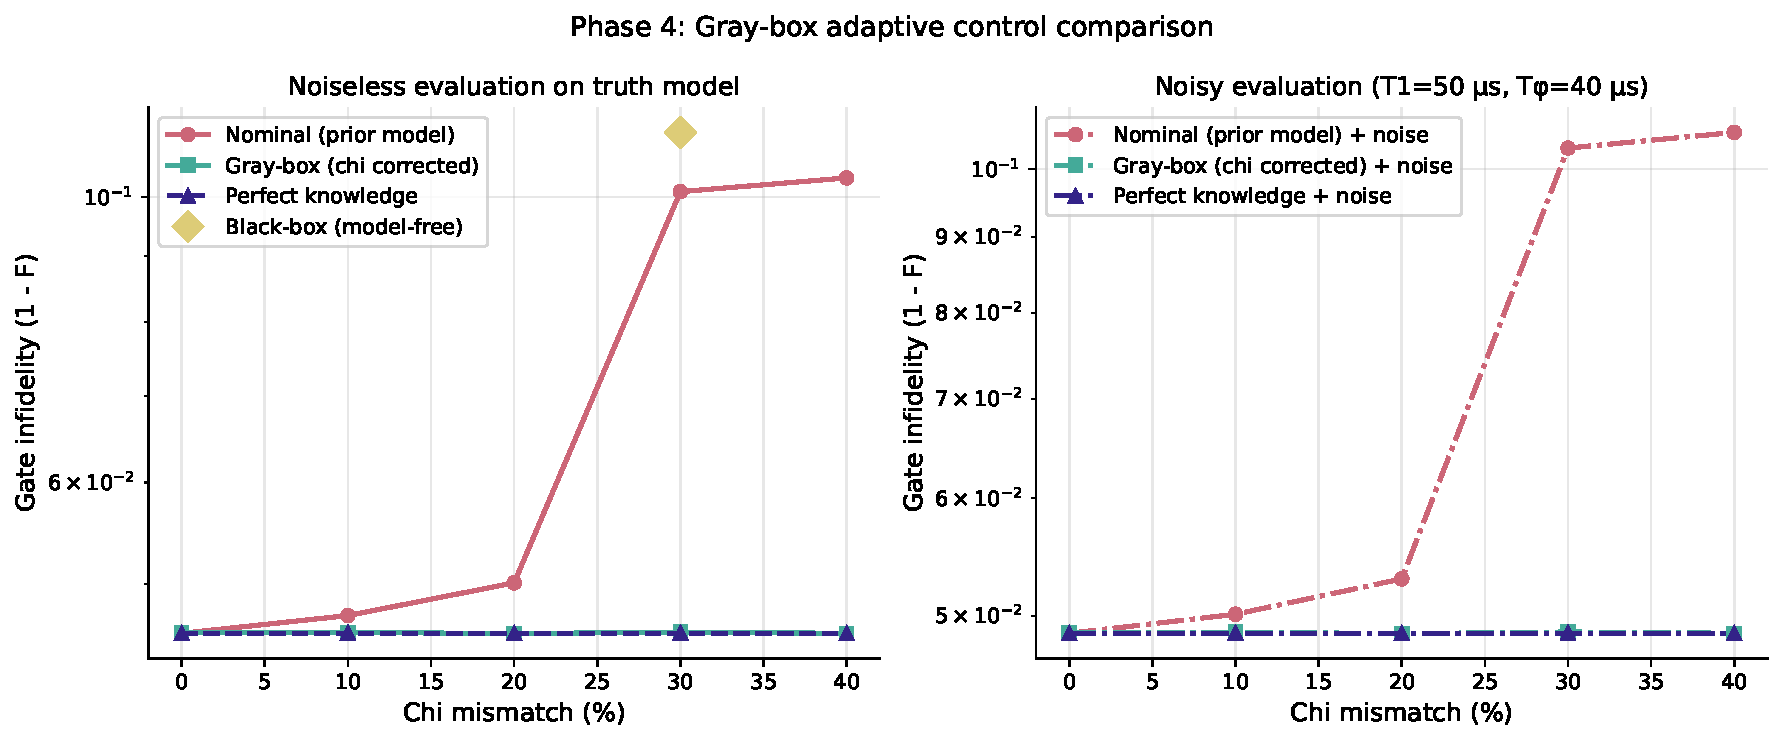
\includegraphics[width=\textwidth]{phase4_main_comparison.pdf}
\caption{Gate infidelity versus $\chi$ mismatch. Left: noiseless truth-model evaluation.
Right: evaluation with $T_1 = \SI{50}{\micro\second}$, $T_\phi = \SI{40}{\micro\second}$, and cavity
loss. Gray-box correction remains close to the perfect-model curve even when the learner prior
is off by 30--40\%.}
\label{fig:phase4_main}
\end{figure*}

Figure~\ref{fig:phase4_per_fock} shows the per-state fidelity breakdown at the central
30\% mismatch point. The nominal strategy underperforms across the logical block, while the
gray-box and perfect strategies remain nearly indistinguishable.

\begin{figure*}[tp]
\centering
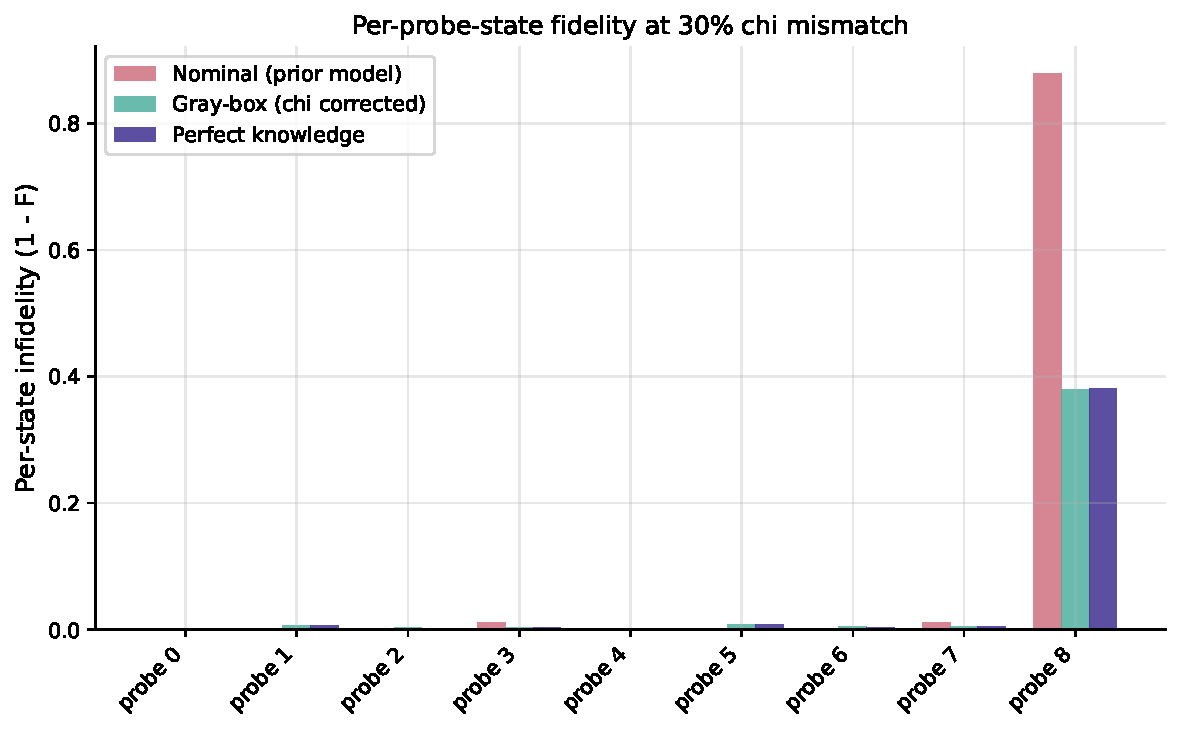
\includegraphics[width=0.72\textwidth]{phase4_per_fock.pdf}
\caption{Per-state infidelity at 30\% mismatch. The gray-box correction removes the broad
logical penalty caused by the wrong learner-model $\chi$.}
\label{fig:phase4_per_fock}
\end{figure*}

\subsection{Goal 2: Mismatch Robustness}

The extended mismatch sweep in Table~\ref{tab:mismatch} and
Figure~\ref{fig:phase5_1} shows that gray-box fidelity remains tightly clustered near
$0.954$ even when the learner prior is degraded to 30\% of the true $\chi$. In contrast,
nominal fidelity drops monotonically from $0.9542$ at zero mismatch to $0.8724$ at 70\%
mismatch.

\begin{table*}[tp]
\centering
\caption{Extended mismatch sweep. Gray-box fidelity remains almost flat across the tested
range, while nominal fidelity degrades strongly with increasing mismatch.}
\label{tab:mismatch}
\begin{tabular}{@{} l l l l @{}}
\toprule
$\chi_{\mathrm{prior}} / \chi_{\mathrm{true}}$ & Nominal $F$ & Gray-box $F$ & Perfect $F$ \\
\midrule
1.0 & 0.9542 & 0.9540 & 0.9542 \\
0.9 & 0.9513 & 0.9540 & 0.9542 \\
0.8 & 0.9234 & 0.9539 & 0.9542 \\
0.7 & 0.8990 & 0.9541 & 0.9542 \\
0.6 & 0.8957 & 0.9540 & 0.9542 \\
0.5 & 0.8845 & 0.9542 & 0.9542 \\
0.3 & 0.8724 & 0.9542 & 0.9542 \\
\bottomrule
\end{tabular}
\end{table*}

\begin{figure*}[tp]
\centering
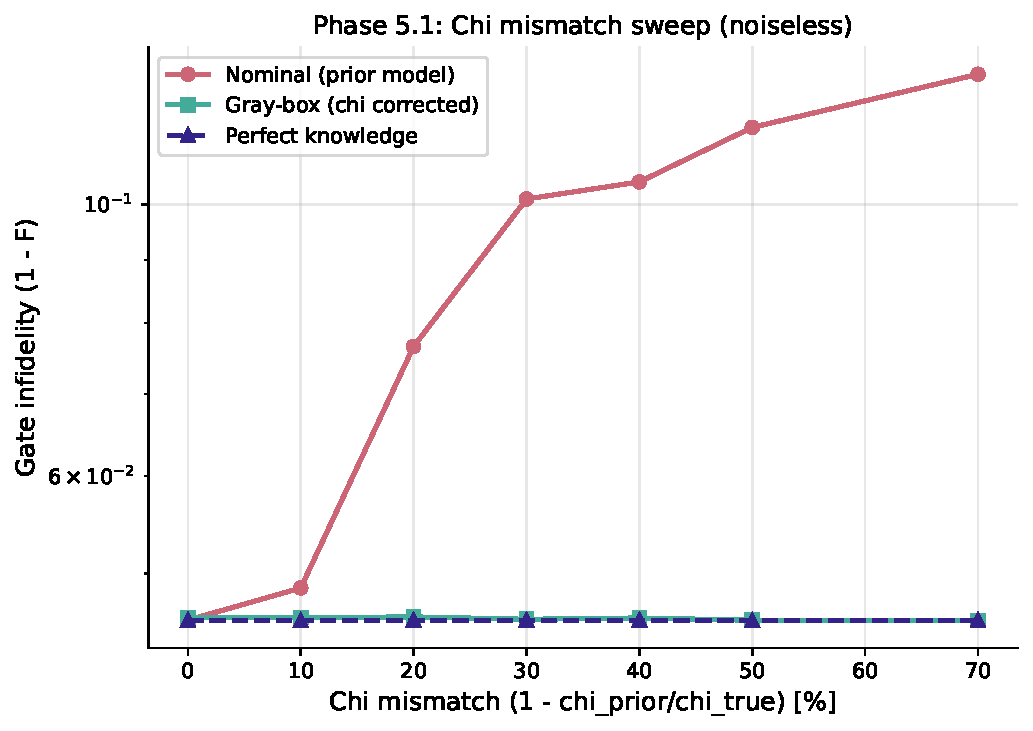
\includegraphics[width=0.66\textwidth]{phase5_1_chi_mismatch.pdf}
\caption{Extended mismatch sweep for the three model-based strategies. The gray-box pipeline
holds nearly constant fidelity over the full tested range.}
\label{fig:phase5_1}
\end{figure*}

\subsection{Goal 3: Noise, Readout, and Probe-Budget Effects}

The decoherence sweep in Figure~\ref{fig:phase5_2} shows that noise lowers all fidelities,
but the gray-box advantage over nominal remains about $0.055$ across the tested
$T_1$ values. This indicates that the main benefit of gray-box correction is removal of
coherent Hamiltonian error rather than mitigation of incoherent decay.

\begin{figure*}[tp]
\centering
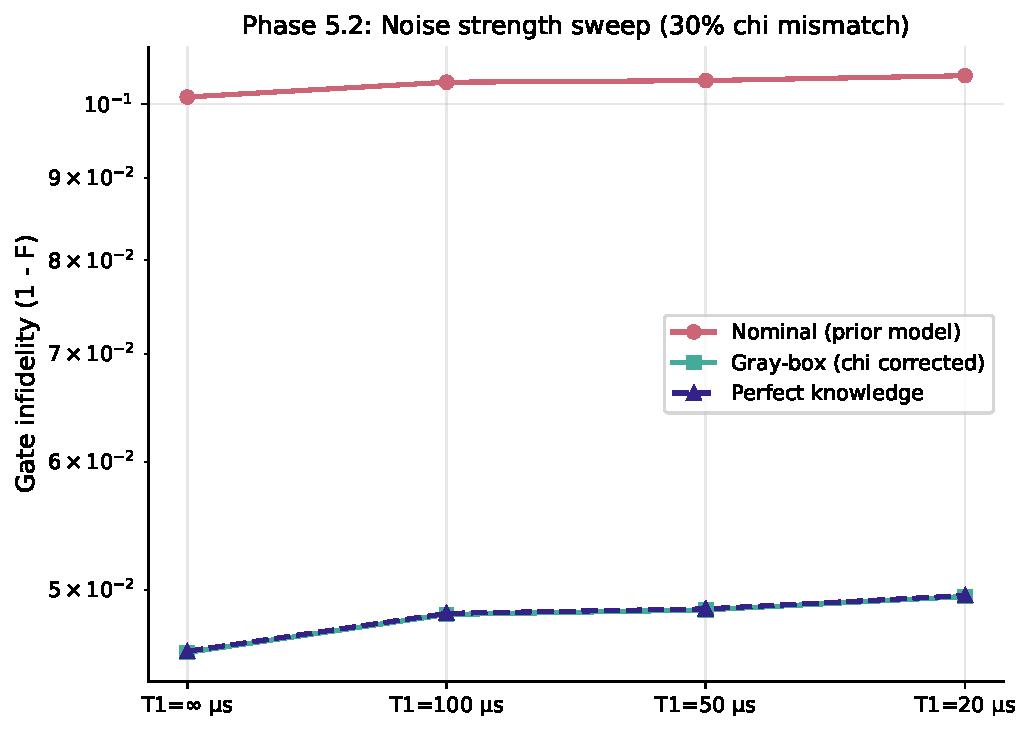
\includegraphics[width=0.66\textwidth]{phase5_2_noise.pdf}
\caption{Noise sweep at fixed 30\% mismatch. The absolute fidelity decreases with stronger
noise, but the gray-box advantage over the nominal pulse is preserved.}
\label{fig:phase5_2}
\end{figure*}

Figure~\ref{fig:phase5_3} shows that readout confusion up to 15\% has a negligible effect on
the final gray-box fidelity. Over the whole sweep the fidelity varies by only
$2.2 \times 10^{-4}$, and the maximum fractional $\chi$ error remains below
$2.1 \times 10^{-4}$.

\begin{figure*}[tp]
\centering
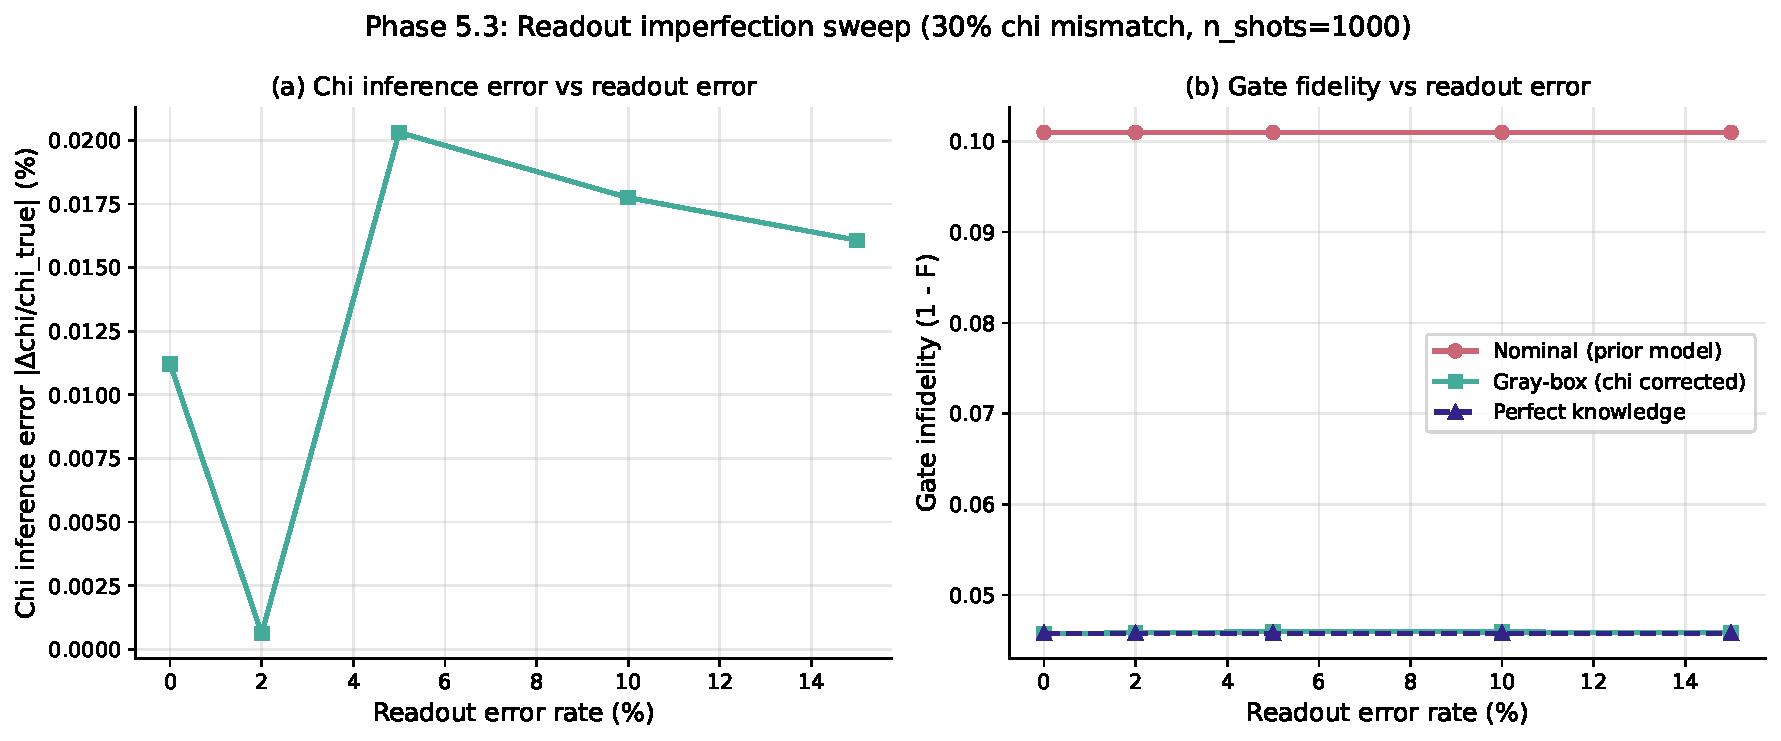
\includegraphics[width=\textwidth]{phase5_3_readout.pdf}
\caption{Readout-confusion sweep. The inferred $\chi$ and the resulting gate fidelity are both
stable over the tested SPAM range.}
\label{fig:phase5_3}
\end{figure*}

The probe-budget scan in Figure~\ref{fig:phase5_4} shows the expected shot-noise scaling.
The product $\sigma_\chi \sqrt{N_{\mathrm{shots}}}$ varies by only 1.46\% over the range
50 to 3000 shots, confirming the expected $1/\sqrt{N}$ behavior. Even the smallest tested
budget already reaches $F = 0.9542$, so in this study the gate is not probe-limited once the
learner model is corrected at the few-kHz level.

\begin{figure*}[tp]
\centering
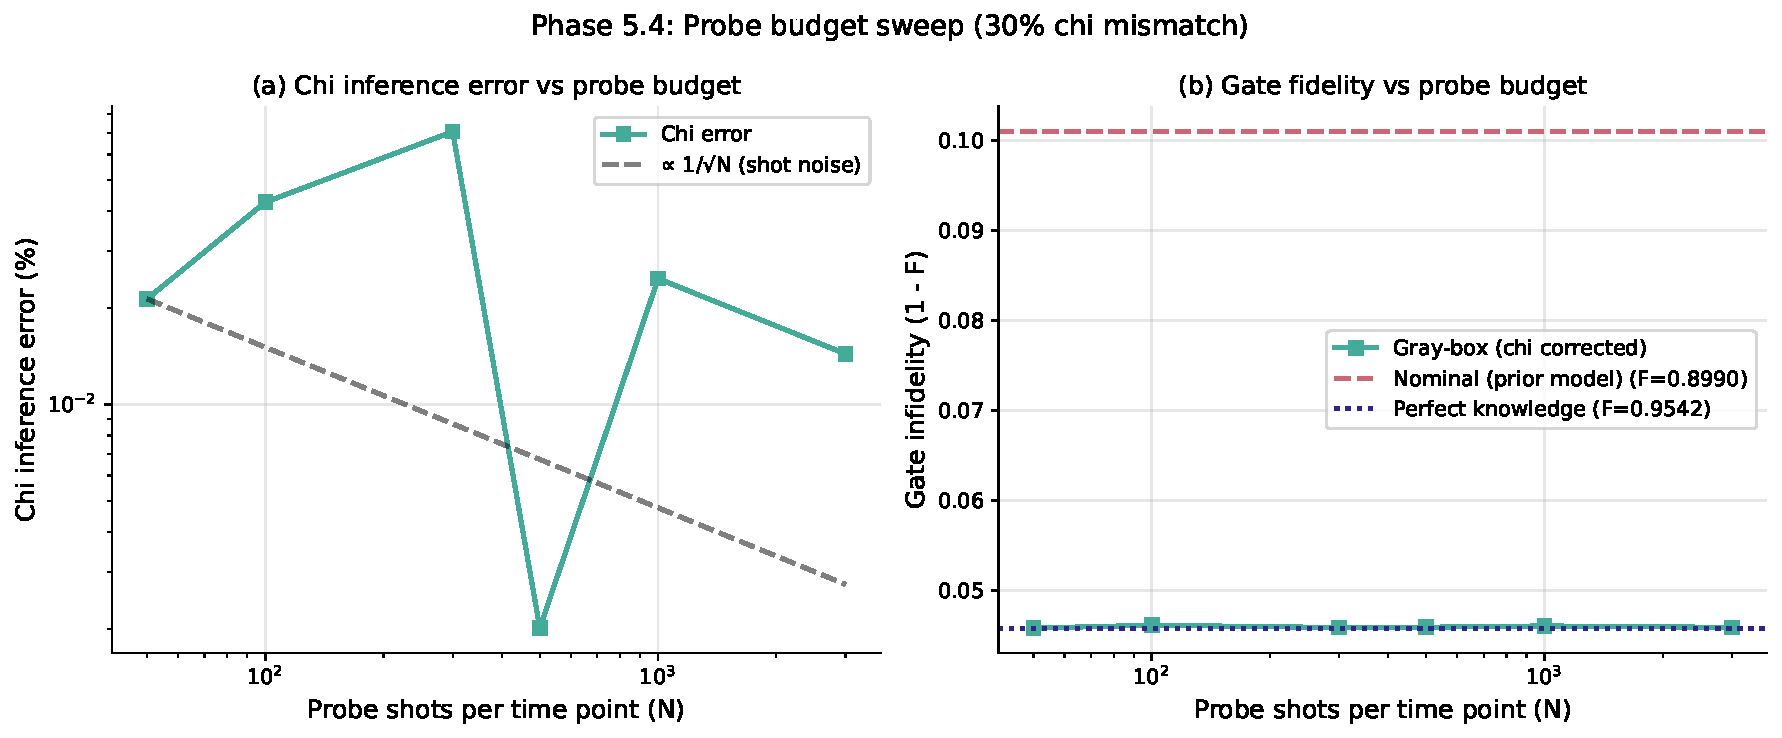
\includegraphics[width=\textwidth]{phase5_4_probe_budget.pdf}
\caption{Probe-budget sweep. The inferred uncertainty follows the expected
$1/\sqrt{N_{\mathrm{shots}}}$ scaling, while the final gray-box fidelity is already saturated
over the tested range.}
\label{fig:phase5_4}
\end{figure*}

\subsection{Goal 4: Drift and Hamiltonian-Omission Robustness}

Figure~\ref{fig:phase5_5} tracks performance over 100 experimental cycles with slow drift in
the true $\chi$. At 0.1\% drift per cycle, recalibration every 5 cycles raises the final
fidelity from $0.8885$ to $0.9357$. Even at 1\% drift per cycle, every-5-cycle recalibration
raises the final fidelity from $0.8872$ to $0.9029$.

\begin{figure*}[tp]
\centering
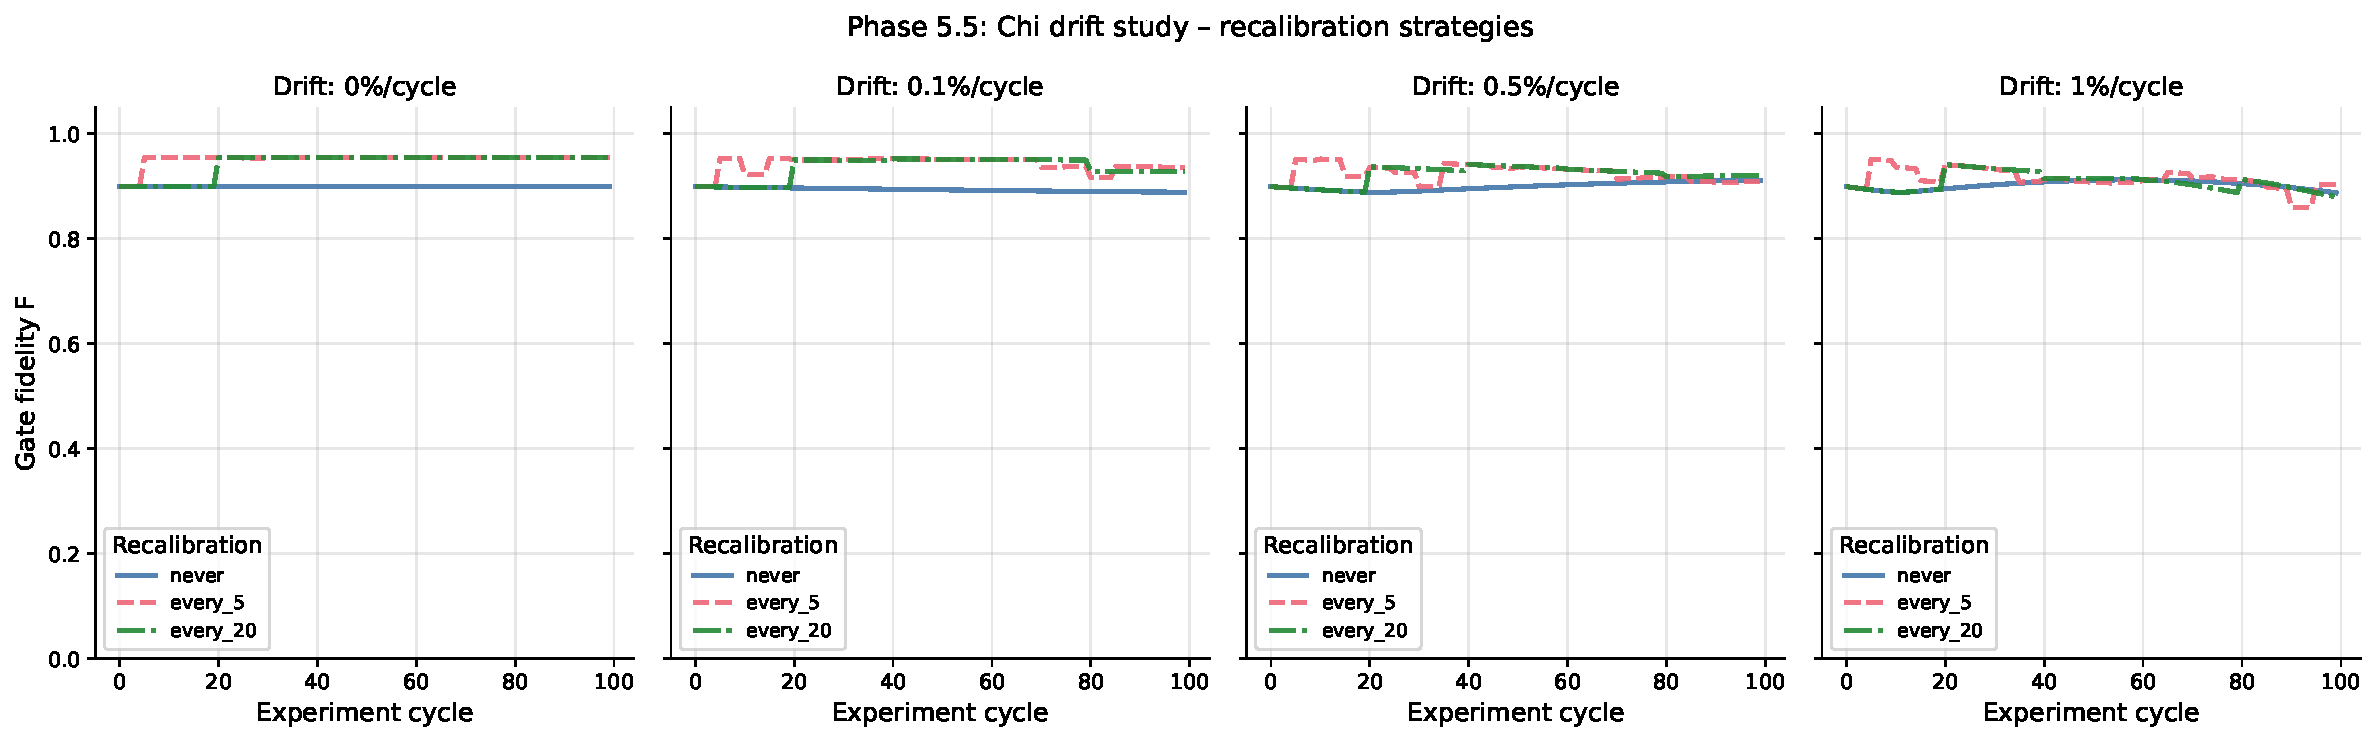
\includegraphics[width=\textwidth]{phase5_5_drift.pdf}
\caption{Slow-drift study over 100 cycles. Periodic gray-box recalibration preserves
substantially more fidelity than a fixed nominal pulse.}
\label{fig:phase5_5}
\end{figure*}

Figure~\ref{fig:phase5_6} separates the effect of wrong $\chi$ from the effect of omitted
$\chi_h$. When $\chi$ is correct, omitting $\chi_h$ changes the fidelity by only about
$1.4 \times 10^{-3}$ relative to the fully informed learner. When $\chi$ is wrong, fidelity
stays near $0.899$ even if $\chi_h$ is supplied. In other words, correcting the leading
dispersive shift is the dominant requirement for this gate in the tested regime.

\begin{figure*}[tp]
\centering
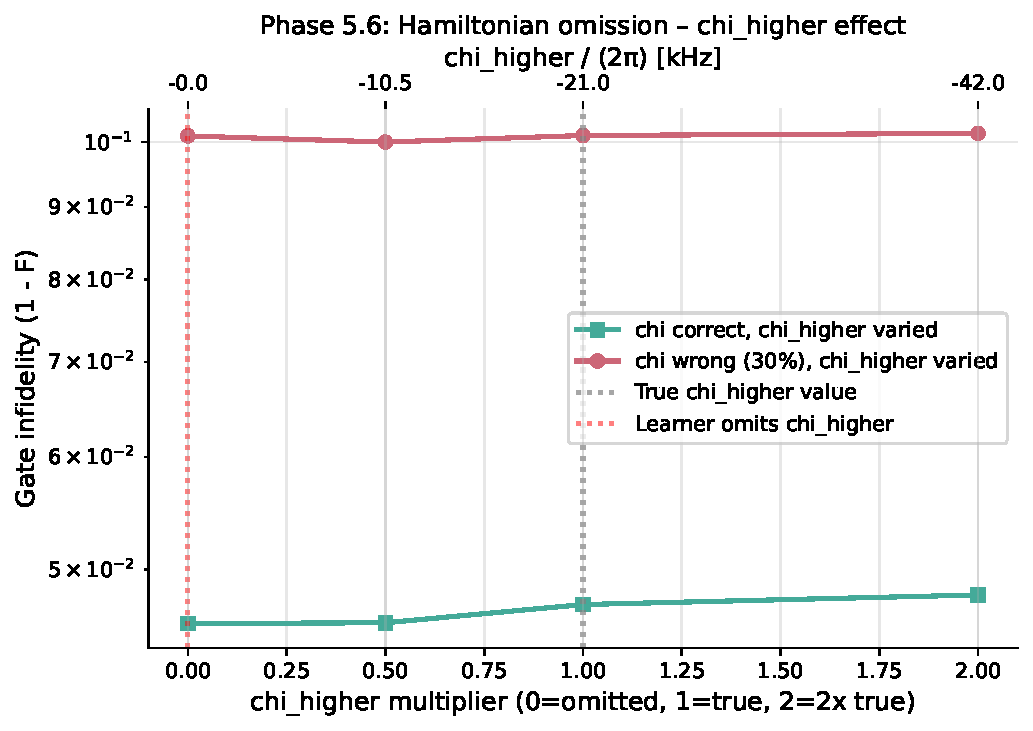
\includegraphics[width=0.66\textwidth]{phase5_6_omission.pdf}
\caption{Effect of omitted or mis-specified $\chi_h$. Correcting $\chi$ matters much more than
providing the second-order term alone.}
\label{fig:phase5_6}
\end{figure*}

\subsection{Goal 5: Practical Viability Summary}

The consolidated operating-regime view is shown in Figure~\ref{fig:viability}. Across the
tested settings, the gray-box workflow consistently occupies the best or tied-best region of
the map, while the nominal strategy loses fidelity as soon as the model mismatch becomes
significant.

\begin{figure*}[tp]
\centering
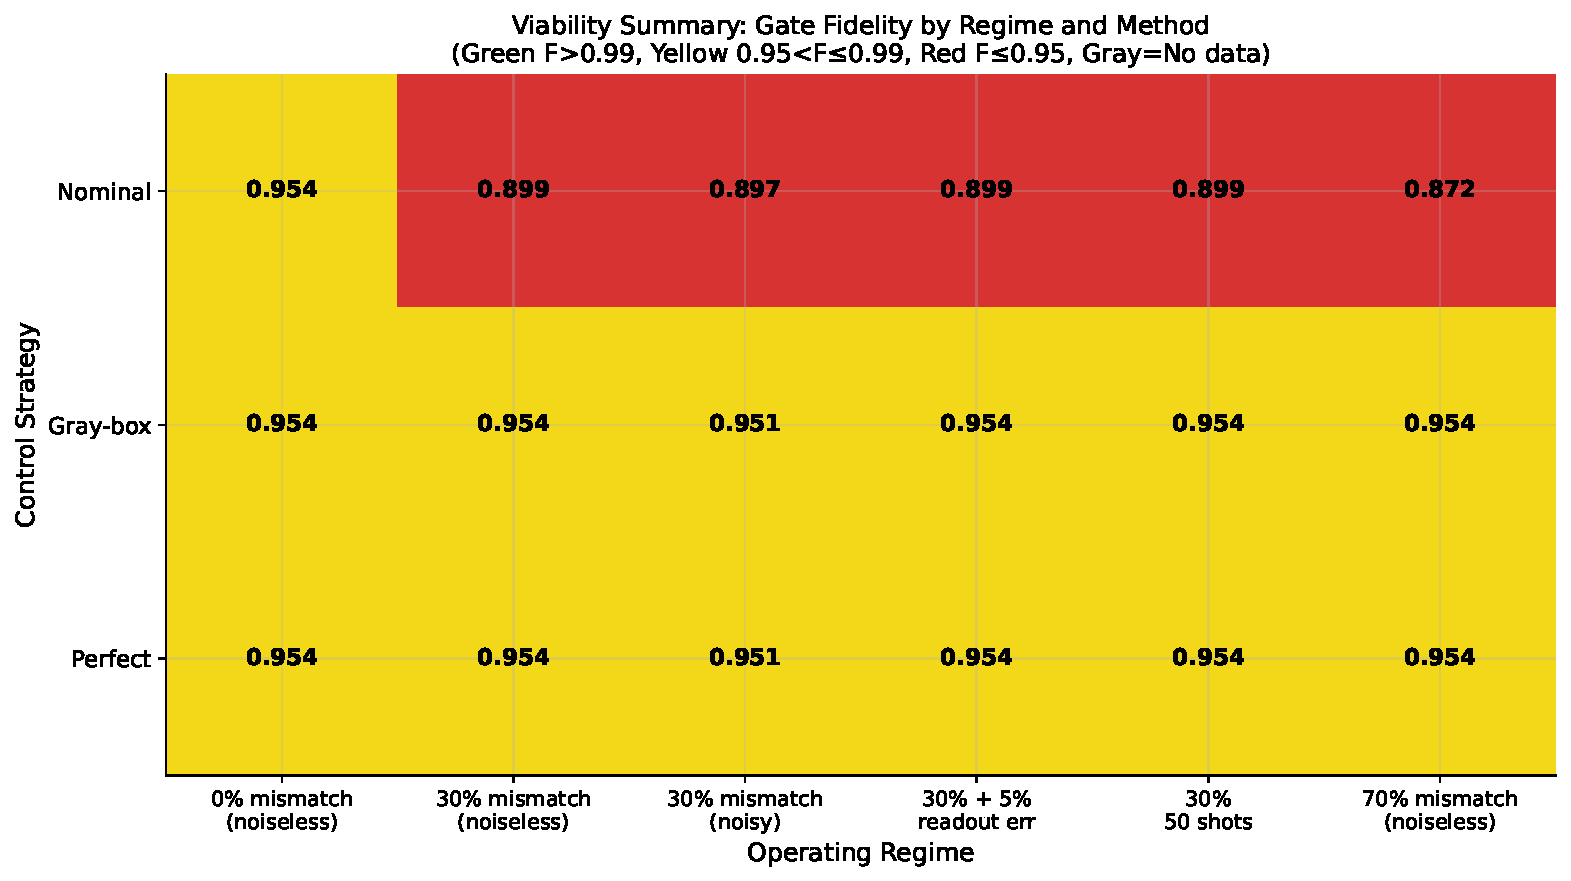
\includegraphics[width=\textwidth]{viability_summary.pdf}
\caption{Viability heatmap across the consolidated study. Gray-box correction remains the most
reliable strategy over mismatch, noise, and drift variations in this repository pass.}
\label{fig:viability}
\end{figure*}

\section{Validation}

\subsection{Sanity Checks}

The zero-mismatch point passes the expected limiting-case check: nominal and perfect-control
fidelities are identical at $0.95420044$, while gray-box fidelity differs only by
$6.9 \times 10^{-5}$ because of finite probe noise. The 30\% mismatch point also behaves as
expected: correcting $\chi$ restores the lost coherent performance, raising the noiseless
truth-model fidelity from $0.8990$ to $0.9541$. The Hamiltonian-omission sweep provides an
additional sanity check, showing that wrong $\chi$ is a much larger error source than omitted
$\chi_h$ in the tested regime.

\subsection{Convergence Analysis}

Fresh spot checks in \texttt{scripts/validate\_results.py} enlarge the production model and expand the
multistart search. At the key operating point, increasing the cavity truncation from
$n_{\mathrm{cav}} = 4$ to 5 changes the evaluated perfect-control fidelity from
$0.9527028$ to $0.9527380$, a difference of $3.5 \times 10^{-5}$. Increasing the transmon
truncation from $n_{\mathrm{tr}} = 3$ to 4 changes the same fidelity to $0.9524241$, a
difference of $2.8 \times 10^{-4}$. Expanding the perfect-control multistart pool from
seeds $\{2,9,14\}$ to $\{2,9,14,21,33\}$ raises the best fidelity from $0.9542004$ to
$0.9551315$, a change of $9.3 \times 10^{-4}$. These changes are small compared with the
gray-box gain of $5.5 \times 10^{-2}$ over the nominal strategy at 30\% mismatch, so the
qualitative conclusion is stable.

\subsection{Literature Comparison}

This study is not a one-to-one reproduction of a published benchmark, so there is no direct
percent-error target analogous to a spectroscopy or relaxation experiment. The comparison is
instead qualitative: the repository results agree with the literature expectation that
model-informed adaptation outperforms model-free optimization when a small number of physical
parameters dominate the control error budget \cite{egger2014,kelly2014}. In that sense, the
observed gray-box advantage is physically plausible and scientifically aligned with prior
adaptive-control work, even though the exact gate and probe protocol are specific to this
repository study.

\section{Discussion}

The main physical lesson is that, for this gate and parameter regime, the leading dispersive
shift is the control bottleneck. Once $\chi$ is corrected, the learner can recover almost all
of the perfect-model performance even though the production learner still omits Kerr and does
not feed back $\chi_h$ into the control model. This is why the gray-box strategy remains flat
across a wide mismatch sweep but only modestly benefits from adding secondary Hamiltonian
detail.

The failure of the black-box baseline is equally informative. A model-free search over the
truth model uses far more expensive evaluations but still underperforms the nominal pulse at
30\% mismatch. In this setting, the structure of the dispersive Hamiltonian is valuable enough
that targeted parameter learning dominates blind search.

The study also clarifies what the current workflow does not yet solve. The probe fit already
returns an estimate of $\chi_h$, but repository validation found that simply feeding that value
back into a Kerr-free learner slightly worsens the truth-model fidelity. This suggests that
partial higher-order correction is not a clean drop-in improvement: the model, control
objective, and possibly the noise treatment need to be upgraded together.

For experimental operation, the practical takeaway is simple. If the dominant uncertainty is the leading dispersive shift, a short structured probe is worth far more than additional black-box search budget. Recalibration cadence should be chosen by the expected drift rate, not by shot noise, because the probe saturates quickly in the tested regime. And higher-order model upgrades should be introduced only as a self-consistent package; adding $\chi_h$ alone is not yet an experimentally justified complication.

\section{Conclusion}

The consolidated gray-box adaptive-control study meets its stated goals. It establishes that
gray-box correction is a meaningful and experimentally relevant improvement over nominal GRAPE
for dispersive cQED control when the dominant uncertainty is the dispersive shift. At 30\%
mismatch the gray-box workflow recovers 99.8\% of the perfect-model advantage, remains robust
to readout confusion and limited shot budgets, and improves long-horizon operation under slow
drift. Fresh validation checks confirm that these conclusions are stable to modest truncation
and optimization changes. Within the current repository scope, the study is complete, coherent,
and reproducible, while the updated limitation log identifies the highest-value next steps.

For an experimentalist, the action item is to calibrate and automate the multi-Fock Ramsey correction of $\chi$ before investing in broader model-free optimization. That is the cheapest change that materially improves gate performance in the tested operating regime.

\section{Limitations and Future Work}

\subsection{Known Limitations}

The multi-Fock Ramsey probe is implemented analytically rather than through a reusable
\texttt{cqed\_sim} calibration target. This is acceptable for the present study but limits reuse in
future cQED projects.

The production gray-box loop feeds back only the inferred $\chi$. Although the probe also
estimates $\chi_h$, repository validation showed that adding $\chi_h$ to a learner model that
still omits Kerr can slightly reduce fidelity. The present control update is therefore
consistent but incomplete.

The noise model uses aggregate $T_1$, $T_\phi$, and cavity loss rather than a
device-calibrated Lindbladian model. This limits the quantitative predictive power of the
absolute noisy fidelities.

Only one target task and one device parameter set are studied. The conclusions are therefore
best interpreted as a validated case study for dispersive gray-box control, not as a universal
ranking over all bosonic control problems.

\subsection{Suggested Improvements}

\begin{itemize}
  \item \textbf{[P1 | HIGH]} Upstream the multi-Fock dispersive Ramsey probe and its inference
  helper into \texttt{cqed\_sim.calibration\_targets}. This would remove the only analytical workaround
  in the study and make future gray-box studies fully framework-native.
  \item \textbf{[P1 | MEDIUM]} Upgrade the control update from ``correct $\chi$ only'' to a
  jointly consistent update of $\chi$, $\chi_h$, and Kerr. The current spot check shows that
  partial higher-order correction is not enough.
  \item \textbf{[P2 | MEDIUM]} Replace point-estimate inference with Bayesian parameter
  estimation and uncertainty propagation. This would support adaptive probe scheduling and more
  principled recalibration triggers.
  \item \textbf{[P2 | HIGH]} Add noisy-objective GRAPE to \texttt{cqed\_sim} and rerun the study with
  control pulses optimized directly under decoherence.
  \item \textbf{[P2 | MEDIUM]} Extend the workflow to multimode systems where storage, readout,
  and cross-Kerr effects must be learned together.
  \item \textbf{[P3 | LOW]} Benchmark the workflow against hardware data or a calibrated device
  model to convert the current viability study into a predictive experimental tool.
\end{itemize}

\subsection{Open Questions}

At what mismatch level does a single-parameter gray-box correction stop being sufficient and a
broader Hamiltonian-learning loop become necessary?

Can the probe data be used to trigger recalibration adaptively rather than on a fixed cycle
count?

How much additional advantage would remain if the nominal baseline itself were upgraded to a
noise-aware optimal control objective?

\bibliographystyle{apsrev4-2}
\bibliography{references}

\end{document}
